\documentclass[11pt, oneside]{article}
\usepackage[margin=1in,letterpaper]{geometry}
\usepackage{times}
\usepackage{graphicx}
\usepackage{amssymb,amsmath,mathtools}
\usepackage{array}
\usepackage{longtable}
\usepackage{color}
\usepackage[T1]{fontenc}
\usepackage{sectsty}
\usepackage[normalem]{ulem}
\usepackage{tikz}
\usetikzlibrary{decorations.pathmorphing,calc,arrows.meta}
\usepackage{float}
\sectionfont{\fontsize{12}{12}\selectfont}
\subsectionfont{\fontsize{11}{11}\selectfont}
\subsubsectionfont{\normalsize\itshape\mdseries}

\renewcommand\labelitemi{{\boldmath$\cdot$}}
% NOTE: dots at every level; the handwritten dashes and arrows are set explicitly with \item[--], \item[$\rightarrow$],
% \item[$\hookrightarrow$].
\renewcommand\labelitemii{\labelitemi}
\renewcommand\labelitemiii{\labelitemi}
\renewcommand\labelitemiv{\labelitemi}

%%%%%%%%%%%%%%%%%%%%%%%%%%%%%%%%%%%%%
% Notation: symbols follow ../variables_master.tex. Renames that apply existing instructor decisions (each also marked
% at first use):
%   - Boltzmann constant K_B -> k_B and free-space wavenumber K_0 -> k_0 (D14);
%   - spectral radiance B_omega -> B_f and spectral power P_omega -> P_f (per unit ordinary frequency f, units per Hz;
%     as B_omega -> B_f in Lecture 12, Eq. e:Bf there);
%   - Stefan-Boltzmann constant sigma -> sigma_SB (D117);
%   - receiving-antenna area A_r -> A_eff (D52: receive areas are written A_eff; the effective aperture, as in U&L
%     2014, Eq. 3.31a, p. 85);
%   - Rayleigh-Jeans expansion variable gamma = hf/(k_B T) -> z, the L12 symbol for the same quantity (D132; gamma is
%     reserved for the propagation constant, D9) (D139, approved 2026-09-30);
%   - optical depth tau -> tau_opt (tau is the Fresnel transmission coefficient, D18; F2 suggestion) (D137, formerly
%     F2; approved 2026-09-30);
%   - underlined position vector r -> bold r (as in L5).
% Kept as handwritten (master table D138-D149, all approved 2026-09-30): brightness I (a radiance, W m^-2 sr^-1) next to
% the L12 flux density I (D138), c_p (D140), A_s, Omega_s, Omega_r (D141), Omega_p (D142), F(theta, phi) (D143),
% spherical angles theta, phi (D144), emissivity e (D145), T_B, T_VS (D146), R-hat (D147), albedo a (D148), source
% functions J, J_a, J_s (D149).
% Descriptive subscripts (s source, r receiver, p pattern, a absorption, s scattering, B brightness, VS volume
% scattered, bb black body, eff, opt) are upright, as in Ulaby & Long; c_p keeps the handwritten italic p.
% Not triggered in this lecture (no mu = cos theta, no asymmetry factor): F6, F11.
% Main reference checks: Ulaby & Long (2014), Secs. 6-1 to 6-6 (pp. 227-243), Eqs. 6.2-6.26, 6.45-6.60, Table 6-1
% (p. 228), Figs. 6-2, 6-4, 6-12; Sec. 3-2 (p. 82), Eq. 3.16; Eq. 3.31a (p. 85). Liou (2002), Sec. 1.1 (pp. 3-5),
% Eqs. 1.1.5-1.1.10; Sec. 1.4 (pp. 27-30), Eqs. 1.4.1-1.4.17.
%%%%%%%%%%%%%%%%%%%%%%%%%%%%%%%%%%%%%

\newcommand{\ke}{\kappa_\mathrm{e}}
\newcommand{\ka}{\kappa_\mathrm{a}}
\newcommand{\ks}{\kappa_\mathrm{s}}
\newcommand{\Aeff}{A_\mathrm{eff}}
\newcommand{\topt}{\tau_\mathrm{opt}}
\newcommand{\rv}{\mathbf{r}}
\newcommand{\Rh}{\hat{\mathbf{R}}}

\title{Ge 158 Lecture 13: Radiometry and Radiative Transfer}
\author{Brent Minchew}
\date{}

\setlength{\emergencystretch}{1.5em}
\renewcommand{\topfraction}{0.85}
\renewcommand{\textfraction}{0.1}
\renewcommand{\floatpagefraction}{0.75}
\begin{document}
\maketitle

\noindent\underline{\textbf{Topics covered}}
\begin{itemize}
	\item Review of black body radiation
	\item Overview of radiometry
	\item Radiative transfer equation
\end{itemize}

%%%%%%%%%%%%%%%%%%%%%%%%%%%%%%%%%%%%%
% ---- page L1 ----
% NOTE: section heading from the handwritten underlined heading "Radiometry" (page L1).
\section{Radiometry}
\label{s:radiometry}

\begin{itemize}
	% NOTE: checked against U&L 2014, p. 227 (Sec. 6-1: radiometry measures incoherent radiant energy).
	\item Remote sensing method for measuring EM radiation from planetary surfaces, atmospheres, and other natural media
	\begin{itemize}
		\item[$\rightarrow$] More specifically, radiometry is measure of \underline{incoherent} radiant EM energy
	\end{itemize}
\end{itemize}

% NOTE: subsection heading added (the topic "Review of black body radiation" is listed on page L0).
\subsection{Review of black body radiation}
\label{s:review}

\begin{itemize}
	% NOTE (page L1): handwritten B_omega; written B_f, per unit ordinary frequency f (the units are per Hz and the
	% right side is a function of f), as in Lecture 12 (Eq. e:Bf there; master table B_f, D129). Checked against U&L
	% 2014, Eq. 6.2 (p. 229; I_f in W m^-2 sr^-1 Hz^-1, h = 6.63e-34 J s, k = 1.38e-23 J/K) and Liou 2002, Eq. 1.2.3 (per-frequency form).
	% Handwritten K_B written k_B (D14).
	\item To get started, recall Planck's law from last lecture
	\begin{equation}
		\label{e:Bf}
		B_f = \frac{2hf^3}{c^2}\left[\frac{1}{e^{hf/k_BT} - 1}\right] \qquad \left[\frac{\text{W}}{\text{m}^2\,\text{sr}\,\text{Hz}}\right] \equiv \text{spectral radiance}
	\end{equation}
	\begin{itemize}
		\item[] $h \equiv$ Planck's const $= 6.63\times10^{-34}$~J$\cdot$s
		\item[] $f = \dfrac{\omega}{2\pi}$
		\item[] $c \equiv$ speed of light
		\item[] $k_B \equiv$ Boltzmann's const $= 1.38\times10^{-23}$~$\dfrac{\text{J}}{\text{K}}$
		\item[] $T \equiv$ absolute temperature
	\end{itemize}
	% NOTE (page L1): handwritten "Wein's" corrected to "Wien's" (Wilhelm Wien; Liou 2002, Sec. 1.2.3, p. 12), as in
	% Lecture 12. "equiv." kept as handwritten: the frequency of the peak of B_f and the wavelength of the peak of
	% B_lambda both scale with T (f_max = 5.879e10 Hz/K x T; lambda_max = b_W/T; python3), but they are not
	% reciprocal: c/f_max ~ 1.76 lambda_max (Lecture 12, NOTE at Eq. e:Wien). Area under B_f: the total radiance L
	% (Lecture 12, Eq. e:Ltot), which scales as T^4.
	\item[--] Recall that when we increase $T$, we increase the frequency of max $B_f$ (equiv., we decrease the wavelength according to $\lambda_\mathrm{max} \sim T^{-1}$ $\rightarrow$ Wien's displacement law) and total radiated power (area under $B_f$ curve)
\end{itemize}

% ---- page L2 ----
\begin{itemize}
	\item How is this used in practice?
	\begin{itemize}
		% NOTE: checked against U&L 2014, p. 231 ("I_f is the power (in watts) emitted by a blackbody source of
		% surface area 1 m^2, through a solid angle of 1 sr, and over a bandwidth of 1 Hz").
		% NOTE: added (instructor decision 2026-09-30): the parenthetical on projected area. Radiance is per unit area
		% projected normal to the direction of emission, cos(theta) dA (Liou 2002, Eqs. 1.1.6-1.1.7, p. 4); for
		% isotropic radiation the hemispheric flux density is then the integral of B cos(theta) dOmega = pi B (Liou
		% Eqs. 1.1.8-1.1.10, p. 5), whereas per unit surface area in every direction it would be 2 pi B.
		\item[$\hookrightarrow$] First note that $B_f$ is the power emitted by a black body with a 1~m$^2$ surface area through a 1~sr solid angle over a bandwidth of 1~Hz (area projected normal to the direction of emission, which is why the flux into a hemisphere is $\pi B_f$ rather than $2\pi B_f$)
		% NOTE (page L2): handwritten P_omega written P_f (per unit f; units W/Hz; U&L 2014: P_f), and the handwritten
		% antenna area A_r written A_eff (master table D52: receive areas are written A_eff; A_r would be the L5
		% reflected-beam area). U&L 2014 call A_r the area of the receiving aperture (Fig. 6-2, p. 232) and, in
		% Sec. 6-3, its effective aperture (p. 232; Eq. 6.21 with Eq. 3.31a, p. 85, Omega_p = lambda^2/A_e); the
		% geometric solid angle Omega_r = A_eff/R^2 is written with the same symbol, as in U&L. A_s, Omega_s, Omega_r
		% are flagged in master table D141. Checked against U&L 2014, Eqs. 6.7-6.10 (p. 231).
		\item[$\hookrightarrow$] Suppose black body has area $A_\mathrm{s}$, the spectral power $P_f$ received by an antenna w/ area $\Aeff$ at a distance $R$ from black-body is
		\begin{equation}
			\label{e:Pf1}
			P_f = B_f A_\mathrm{s} \Omega_\mathrm{r} \qquad \left[\frac{\text{W}}{\text{Hz}}\right]
		\end{equation}
		where $\Omega_\mathrm{r} = \dfrac{\Aeff}{R^2}$ is solid angle subtended by the antenna
		\item[$\hookrightarrow$] Now note that source area subtends a solid angle $\Omega_\mathrm{s} = \dfrac{A_\mathrm{s}}{R^2}$
		\begin{equation*}
			\Rightarrow\quad R^2 = \frac{\Aeff}{\Omega_\mathrm{r}} = \frac{A_\mathrm{s}}{\Omega_\mathrm{s}}
		\end{equation*}
		and
		\begin{equation}
			\label{e:Pf2}
			P_f = B_f\Aeff\Omega_\mathrm{s}
		\end{equation}
		% NOTE: checked against U&L 2014, Eq. 6.11 (p. 231).
		\item[$\hookrightarrow$] Total power received by a receiver w/ bandwidth $\Delta f = f_\mathrm{high} - f_\mathrm{low}$
		\begin{equation}
			\label{e:Ptot}
			P = \int_{f_\mathrm{low}}^{f_\mathrm{high}} P_f\,df = \Aeff\Omega_\mathrm{s}\int_{f_\mathrm{low}}^{f_\mathrm{high}} B_f\,df
		\end{equation}
		% ---- page L3 ----
		% NOTE (page L3): handwritten reads "P ~= total intensity of black body given by Stephan-Boltzmann Law (see
		% Lecture 12)" and "I ~= pi P = sigma T^4"; corrected to P/(A_eff Omega_s) in both places, because P is a
		% power (W; Eq. e:Ptot) while I = sigma_SB T^4 is a power per unit area (W/m^2): for a band covering the
		% spectrum, Eq. (e:Ptot) gives P -> A_eff Omega_s L, with L the total radiant intensity (radiance) of Lecture 12
		% (Eq. e:Ltot there; W m^-2 sr^-1), so P/(A_eff Omega_s) ~= L and I = pi L (Lecture 12, Eq. e:SB; Liou 2002,
		% Eq. 1.1.10, p. 5, F = pi I for isotropic radiation). The chain "~= ... =" is kept. Handwritten "~= total
		% intensity of black body given by Stefan-Boltzmann Law" changed to "~= total radiance L of black body, and the
		% intensity I = pi L is given by the Stefan-Boltzmann Law" because "total intensity" named L (a radiance) while
		% Eq. (e:SB) gives I = pi L (instructor decision 2026-09-30; Lecture 12, Eqs. e:Ltot, e:SB). Evidence: dimensional analysis, U&L 2014, Eq. 6.11 (p. 231), python3 (pi times the
		% integral of B_f over f at 300 K equals sigma_SB T^4 to 1e-15). "Stephan" corrected to "Stefan" (Josef
		% Stefan; the handwriting itself has "Stefan" two lines below). Handwritten sigma written sigma_SB (D117). I
		% here is the flux density of Lecture 12 (power per unit area, D123, D134); from page L7 on, I is the
		% brightness, a radiance (master table D138).
		\item[$\hookrightarrow$] For sufficiently large $\Delta f$ and an appropriate center frequency, $P/(\Aeff\Omega_\mathrm{s}) \approx$ total radiance $L$ of black body, and the intensity $I = \pi L$ is given by Stefan--Boltzmann Law (see Lecture~12)
		\begin{equation}
			\label{e:SB}
			I \approx \frac{\pi P}{\Aeff\Omega_\mathrm{s}} = \sigma_\mathrm{SB}T^4
		\end{equation}
		% NOTE: added (instructor decision 2026-09-30): the qualifier below. Eq. (e:Ptot) carries no polarization
		% factor, i.e., c_p = 1 in Eq. (e:P); for c_p = 1/2 the same band-integrated power gives
		% pi P/(A_eff Omega_s) = sigma_SB T^4/2 (U&L 2014, p. 233).
		(non-polarized, i.e., dual-polarization, antenna, $c_p = 1$ in Eq.~\eqref{e:P}; a single-polarization antenna receives half)\\
		where
		\begin{equation*}
			\sigma_\mathrm{SB} \equiv \text{Stefan--Boltzmann const} = 5.67\times10^{-8}\left[\frac{\text{W}}{\text{m}^2\text{K}^4}\right]
		\end{equation*}
		% NOTE: the handwritten mark before this line is a star.
		\item[$\bigstar$] But be careful, some RS instruments have narrow bandwidths $\Rightarrow$ Stefan--Boltzmann may not apply
	\end{itemize}
	\item For relatively narrow bands of most RS instruments, must consider Planck's law or an approximation of it
	\begin{itemize}
		\item[$\rightarrow$] at infrared frequencies, it may be advisable to use Planck's law
		% NOTE: checked against U&L 2014, Eq. 6.13 (p. 231), B_f = 2 k_B T f^2/c^2 = 2 k_B T/lambda^2 (K_B written k_B,
		% D14; B_omega written B_f). Scope (NOTE only): U&L, Eq. 6.14b (p. 231), give f/T < 3.9e8 Hz/K as a sufficient
		% condition for a deviation below 1% (python3: with the deviation defined as (RJ - B)/RJ, 0.93% at 3.9e8 Hz/K and 1% at 4.18e8 Hz/K;
		% defined as (RJ - B)/B, 0.94% and 1% at 4.14e8 Hz/K); it fails for
		% the 2.7 K cosmic background at microwave frequencies (U&L p. 231; python3: 9% error at 10 GHz, 2.7 K).
		\item[$\rightarrow$] at microwave frequencies can use Rayleigh--Jeans law
		\begin{equation}
			\label{e:RJ}
			B_f = \frac{2k_BTf^2}{c^2}
		\end{equation}
	\end{itemize}
\end{itemize}

% NOTE (page L3): the handwritten aside is enclosed in square brackets (not a box); set as such.
% NOTE: the handwritten gamma (= hf/k_B T) is written z, the Lecture 12 symbol for the same quantity (Eq. e:Ltot
% there, z = hc/(lambda k_B T); master table D132), because gamma is reserved for the propagation constant (D9);
% flagged as D139.
% NOTE: handwritten reads e^gamma - 1 = (1 + gamma + gamma^2/2!) - 1; corrected by adding "+ ..." inside the
% parentheses, because the truncated series is not equal to e^gamma (U&L 2014, Eq. 6.12, p. 231, has "+ ...").
% "approx z for z << 1" kept as written (an approximation, not a limit). python3: e^z - 1 = 0.010050 at z = 0.01.
\noindent\hspace*{2.2em}$\left[\;\begin{minipage}{0.84\linewidth}
To get Rayleigh--Jeans from Planck's consider identity
\begin{align*}
	e^z - 1 &= \left(1 + z + \frac{z^2}{2!} + \ldots\right) - 1 \qquad \left(\text{where } z = \frac{hf}{k_BT}\right)\\
	&\approx z \quad \text{for } z \ll 1 \rightarrow \text{low frequency limit for which Rayleigh--Jeans applies}
\end{align*}
\end{minipage}\;\right]$

%%%%%%%%%%%%%%%%%%%%%%%%%%%%%%%%%%%%%
% ---- page L4 ----
% NOTE: subsection heading added.
\subsection{Antenna directionality and the power--temperature correspondence}
\label{s:antenna}

\begin{itemize}
	% NOTE: checked against U&L 2014, Sec. 6-3 (p. 232) and Fig. 6-4. U&L, Sec. 3-2 (pp. 81-82): F(theta, phi) is the
	% normalized radiation intensity (normalized pattern; F_max = 1), so "antenna gain as a function of direction" is
	% the gain normalized by its maximum. Handwritten "represents the antenna gain" corrected to "represents the
	% normalized radiation intensity (the antenna gain pattern normalized to a maximum of 1)" (instructor decision,
	% 2026-09-30); the gain G itself includes the radiation efficiency and its peak is not 1 (U&L Sec. 3-2.4, pp. 83-84, Eqs. 3.22-3.24).
	% F, theta, phi: master table D143, D144.
	\item To understand relationship between power received by radiometer and the temperature of source body, we must account for directionality of antenna that has a radiation pattern represented by an arbitrary function $F(\theta,\phi)$ where $\theta$ is the colatitude and $\phi$ the longitude (spherical coordinates)
	\begin{itemize}
		\item[] $F(\theta,\phi)$ represents the normalized radiation intensity (the antenna gain pattern normalized to a maximum of 1) as a function of direction
		\begin{itemize}
			\item[$\rightarrow$] In the case of radiometry, $F(\theta,\phi)$ indicates the antenna's ability to convert EM radiation coming from direction defined by $\theta$ and $\phi$ into electrical power (signal)
		\end{itemize}
	\end{itemize}
	% NOTE: added "(Figure~\ref{f:antenna})".
	\item Most RS antenna will have a lobe structure to the radiation pattern $\Rightarrow$ observational geometry (Figure~\ref{f:antenna})
\end{itemize}

\begin{figure}[!htbp]
	\centering
	% Reproduces the handwritten sketch (page L4), element by element: z axis up (arrowhead), x axis toward the lower left
	% (arrowhead), y axis toward the lower right (arrowhead) (handwritten capitals Z, X, Y written as the coordinates z,
	% x, y); a main lobe (teardrop) rising from the origin along z; small side lobes at the origin; a narrow beam (two
	% lines, no arrowhead) from the origin toward the upper right, ending in a small ellipse, labeled B_f(theta, phi)
	% (handwritten B_omega) by a short leader ending in an arrowhead inside the beam-end ellipse; the angle theta (arc) between the z axis and the beam; a dashed line from
	% the top of the beam down to the x-y plane (drawn vertical, parallel to z; slightly slanted in the scan); a line from the origin to the foot of the dashed line (arrowhead at the
	% foot); the angle phi (arc) between the x axis and that line; labels "main lobe", "side lobes" and F(theta, phi)
	% with curved arrows to the main lobe, the side lobes and the edge of the main lobe.
	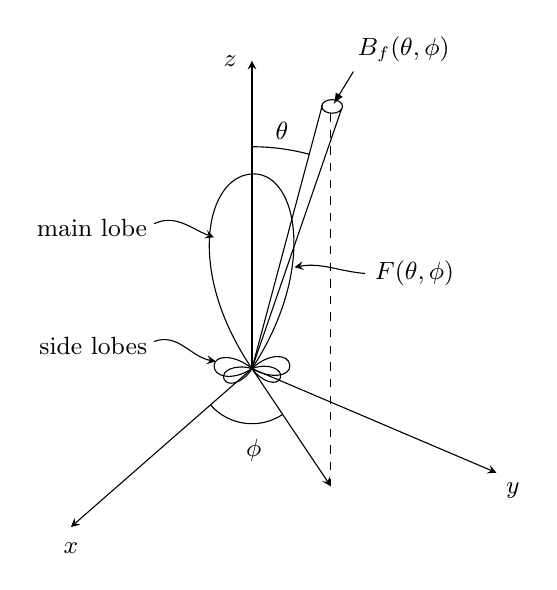
\begin{tikzpicture}[scale=1.15, >=stealth, font=\small]
		\coordinate (O) at (0,0);
		% axes
		\draw[->] (O) -- (0,3.4) node[anchor=east, xshift=-2pt] {$z$};
		\draw[->] (O) -- (-2.0,-1.75) node[anchor=north, yshift=-2pt] {$x$};
		\draw[->] (O) -- (2.7,-1.15) node[anchor=north west] {$y$};
		% main lobe
		\draw (O) .. controls (-0.75,1.1) and (-0.5,2.15) .. (0.02,2.15) .. controls (0.5,2.15) and (0.72,1.1) .. (O);
		% side lobes
		\draw[rotate=175] (O) .. controls (0.2,0.16) and (0.42,0.13) .. (0.42,0) .. controls (0.42,-0.12) and (0.2,-0.14) .. (O);
		\draw[rotate=200] (O) .. controls (0.15,0.12) and (0.33,0.1) .. (0.33,0) .. controls (0.33,-0.1) and (0.15,-0.11) .. (O);
		\draw[rotate=5] (O) .. controls (0.2,0.16) and (0.42,0.13) .. (0.42,0) .. controls (0.42,-0.12) and (0.2,-0.14) .. (O);
		\draw[rotate=-18] (O) .. controls (0.15,0.12) and (0.33,0.1) .. (0.33,0) .. controls (0.33,-0.1) and (0.15,-0.11) .. (O);
		% beam toward the upper right, ending in a small ellipse
		\draw (O) -- (0.78,2.92);
		\draw (O) -- (0.99,2.87);
		\draw (0.885,2.895) ellipse (0.115 and 0.075);
		\draw[<-, >=latex] (0.90,2.92) -- (1.12,3.28) node[anchor=south west, xshift=-2pt] {$B_f(\theta,\phi)$};
		% dashed drop line and its projection on the x-y plane
		\draw[dashed] (0.87,2.82) -- (0.87,-1.3);
		\draw[->] (O) -- (0.87,-1.3);
		% theta
		\draw (0,2.45) arc[start angle=90, end angle=75.0, radius=2.45];
		\node at (0.33,2.63) {$\theta$};
		% phi
		\draw (O) ++(221.2:0.609) arc[start angle=221.2, end angle=303.8, radius=0.609];
		\node at (0.02,-0.9) {$\phi$};
		% labels
		\node[anchor=east] at (-1.05,1.55) {main lobe};
		\draw[->] (-1.08,1.6) to[out=25, in=160] (-0.42,1.45);
		\node[anchor=east] at (-1.05,0.25) {side lobes};
		\draw[->] (-1.08,0.3) to[out=20, in=170] (-0.4,0.08);
		\node[anchor=west] at (1.25,1.05) {$F(\theta,\phi)$};
		\draw[->] (1.25,1.05) to[out=175, in=10] (0.47,1.12);
	\end{tikzpicture}
	\caption{Observational geometry of a radiometer antenna with radiation pattern $F(\theta,\phi)$ (main lobe and side lobes) receiving spectral radiance $B_f(\theta,\phi)$ from the direction $(\theta,\phi)$ (cf.\ Ulaby and Long (2014), Fig.~6-4).}
	\label{f:antenna}
\end{figure}
% NOTE: the caption is added.

% ---- page L5 ----
\begin{itemize}
	% NOTE: checked against U&L 2014, Eqs. 6.15-6.17 (p. 233). Handwritten B_omega, P_omega, A_r written B_f, P_f,
	% A_eff (see above). c_p is flagged against the specific heat c_p of Lecture 10 (master table D140).
	\item To account for antenna directionality let's consider the differential spectral power
	\begin{equation}
		\label{e:dPf}
		dP_f = B_f\Aeff F(\theta,\phi)\,d\Omega
	\end{equation}
	Then the total power received by antenna over bandwidth $\Delta f = f_2 - f_1$
	\begin{equation}
		\label{e:P}
		P = c_p\Aeff\int_{f_1}^{f_2}\iint_{4\pi} B_f F(\theta,\phi)\,d\Omega\,df
	\end{equation}
	where $c_p$ accounts for polarization of antenna
	\begin{equation*}
		c_p = \begin{cases} 1 & \text{non-polarized antenna}\\[2pt] \dfrac{1}{2} & \text{polarized antenna} \end{cases}
	\end{equation*}
	% NOTE: checked against U&L 2014, p. 233 (on average, half of the energy radiated by a black body is polarized
	% along any specified direction).
	Why does $c_p = \frac{1}{2}$ for polarized antenna?
	\begin{itemize}
		\item[] Because EM wave can be represented by two orthogonal polarizations, each w/ half of the total power. (Think: polarized sunglasses) Black bodies radiate unpolarized EM energy $\Rightarrow$ polarizing filter cuts total power in half
	\end{itemize}
\end{itemize}

% ---- page L6 ----
\begin{itemize}
	% NOTE: checked against U&L 2014, Eq. 6.18 (p. 233), with the Rayleigh-Jeans law (Eq. e:RJ), 2 k_B T f^2/c^2 =
	% 2 k_B T/lambda^2. "(which is true for microwaves)" kept as handwritten; see the NOTE at Eq. (e:RJ) for its scope.
	% NOTE: added (instructor decision 2026-09-30): "(antenna inside a black-body enclosure at uniform T)". Taking
	% 2 k_B T/lambda^2 outside the integral over 4 pi requires the black body to fill the whole antenna pattern at one
	% T: U&L 2014, Fig. 6-5a (p. 234), "Antenna inside a blackbody enclosure"; p. 233.
	\item Now assuming Rayleigh--Jeans law is a valid approximation (which is true for microwaves), total power received from a black-body (antenna inside a black-body enclosure at uniform $T$; Ulaby and Long, 2014, Fig.~6-5a)
	\begin{equation}
		\label{e:Pbb1}
		P_\mathrm{bb} = c_p\Aeff\int_{f_1}^{f_2}\iint_{4\pi}\frac{2k_BT}{\lambda^2}F(\theta,\phi)\,d\Omega\,df
	\end{equation}
	% NOTE: checked against U&L 2014, Eqs. 6.19-6.20 (p. 233) and Eq. 3.16 (p. 82). The underbrace is handwritten.
	\item Taking the common case in RS of a narrow bandwidth where $B_f \approx$ constant over $\Delta f$
	\begin{equation}
		\label{e:Pbb2}
		P_\mathrm{bb} = k_BT\Delta f\,\frac{\Aeff}{\lambda^2}\underbrace{\iint_{4\pi}F(\theta,\phi)\,d\Omega}_{\mathclap{=\,\Omega_\mathrm{p}\,\equiv\,\text{antenna pattern solid angle}}} \qquad \text{for } c_p = \frac{1}{2}
	\end{equation}
	% NOTE: checked against U&L 2014, Eq. 6.21 (p. 233) and Eq. 3.31a (p. 85; lossless antenna, effective aperture
	% A_e). Omega_p is flagged in master table D142. The box is handwritten. python3: an isotropic pattern (F = 1)
	% gives Omega_p = 4 pi.
	\item From antenna theory (Ulaby and Long, 2014, ch.~3)
	\begin{equation}
		\label{e:Op}
		\Omega_\mathrm{p} = \frac{\lambda^2}{\Aeff}
	\end{equation}
	% NOTE: checked against U&L 2014, Eq. 6.22 (p. 233), P_bb = kTB (their B is the bandwidth Delta f here).
	\begin{equation}
		\label{e:Pbb}
		\Rightarrow\quad \boxed{P_\mathrm{bb} = k_BT\Delta f}
	\end{equation}
	$\rightarrow$ power received at antenna is proportional to $T$ w/ const of proportionality $= k_B\Delta f$ (one a universal const the other an instrument parameter, both known)\\
	$\Rightarrow$ common in radiometry to interchange terms `power' and `temperature'
\end{itemize}

%%%%%%%%%%%%%%%%%%%%%%%%%%%%%%%%%%%%%
% ---- page L7 ----
% NOTE: subsection heading added.
\subsection{Brightness temperature and emissivity}
\label{s:tb}

\begin{itemize}
	% NOTE: checked against U&L 2014, p. 234 ("Real materials, sometimes referred to as gray bodies, emit less than a
	% blackbody does").
	\item Now, a black-body is an idealized material; Real materials emit less radiation than black bodies (called gray bodies; white bodies reflect all incident radiation)
	\item And in RS applications, it is often the case that observed EM radiation has propagated through some medium (e.g., we may be interested in the $T$ of a fire as seen from a satellite) that absorbs and/or scatters EM radiation
	\item Let's take each of these factors in kind
	% NOTE (page L7): checked against U&L 2014, Eqs. 6.24-6.26 (p. 234; their bandwidth B is Delta f here). I(theta,
	% phi) is the brightness (U&L: "brightness intensity"), a radiance in W m^-2 sr^-1 (U&L Table 6-1, p. 228): here
	% P_bb/lambda^2 = P_bb/(A_eff Omega_p) (Eq. e:Op) is a power per unit area per unit solid angle. It is the
	% brightness of one polarization, integrated over the bandwidth Delta f: P_bb = k_B T Delta f (Eq. e:Pbb) holds
	% for c_p = 1/2, and U&L (p. 234, Eq. 6.24) obtain I_bb = k T B/lambda^2 from the Rayleigh-Jeans law by
	% "multiplying it by a factor of 1/2" ("singularly polarized brightness intensity"), i.e., I_bb = (1/2) B_f
	% Delta f. (U&L's printed middle term, I_bb = I_f B, omits this 1/2: with Eq. 6.13, I_f B = 2kTB/lambda^2; book
	% error, not propagated.) The parenthetical "(for one polarization)" after the equation is added (P_bb = k_B T Delta f,
	% Eq. e:Pbb, holds for c_p = 1/2). I is flagged against the
	% Lecture 12 intensity (flux density) in master table D138; e, T_B in D145, D146.
	\item Let us consider a semi-infinite material w/ brightness (intensity) $I(\theta,\phi)$ and physical (or actual) temperature $T$. The observed brightness
	\begin{align}
		I(\theta,\phi) &= e(\theta,\phi)\,\frac{P_\mathrm{bb}}{\lambda^2} \nonumber\\
		&= \frac{k_B}{\lambda^2}\,\Delta f\,e(\theta,\phi)\,T = \frac{k_B}{\lambda^2}\,\Delta f\,T_\mathrm{B}(\theta,\phi) \label{e:I}
	\end{align}
	(for one polarization)\\
	where
	\begin{itemize}
		% NOTE: added (instructor decision 2026-09-30): "(homogeneous, isothermal medium)". U&L 2014, p. 235:
		% "Implied in this definition of emissivity is the assumption that the material is homogeneous and of uniform
		% temperature."
		\item[] $T_\mathrm{B} = eT \equiv$ brightness temperature (homogeneous, isothermal medium; Ulaby and Long, 2014, p.~235)
		\item[] $e(\theta,\phi) \equiv$ emissivity, defines material's ability to emit EM radiation
	\end{itemize}
\end{itemize}

% ---- page L8 ----
\begin{itemize}
	% NOTE: checked against U&L 2014, Eq. 6.26 (p. 234) and p. 235 (0 <= e <= 1). The arrows and labels under the
	% inequality are handwritten. "(per unit area)" kept as handwritten; I is also per unit solid angle (see the NOTE
	% at Eq. e:I). P(theta, phi) is the power received from the material.
	\item In terms of power (per unit area), emissivity is
	\begin{equation}
		\label{e:e}
		e(\theta,\phi) = \frac{I(\theta,\phi)}{I_\mathrm{bb}} = \frac{P(\theta,\phi)}{P_\mathrm{bb}}
	\end{equation}
	\begin{center}
	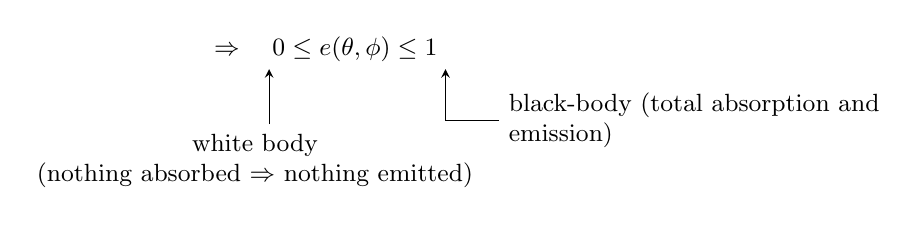
\begin{tikzpicture}[>=stealth, font=\small, baseline]
		\node (ineq) at (0,0) {$\Rightarrow\quad 0 \le e(\theta,\phi) \le 1$};
		\coordinate (zero) at (-0.72,-0.25);
		\coordinate (one) at (1.52,-0.25);
		\draw[->] (-0.72,-0.95) -- (zero);
		\node[anchor=north, align=center] at (-0.9,-0.95) {white body\\(nothing absorbed $\Rightarrow$ nothing emitted)};
		\draw[->] (2.2,-0.9) -- (1.52,-0.9) -- (one);
		\node[anchor=west, align=left] at (2.2,-0.9) {black-body (total absorption and\\emission)};
	\end{tikzpicture}
	\end{center}
	% NOTE: added (instructor decision 2026-09-30): "(in the Rayleigh--Jeans regime, Eq. e:I)". With Planck's law,
	% T_B is not proportional to I: python3, at 10 um and 300 K, z = 4.80 and B/RJ = 0.040.
	\item Brightness temperature often used as a proxy for observed brightness and (equiv.) power because of the proportional relation w/ a known constant of proportionality (in the Rayleigh--Jeans regime, Eq.~\eqref{e:I})
	% NOTE: checked against U&L 2014, p. 235 ("we will henceforth use T_B(theta, phi) as a surrogate for I(theta,
	% phi)").
	\item Let us relate $T_\mathrm{B}$ to the physical and dielectric properties of the material and atmosphere
\end{itemize}

%%%%%%%%%%%%%%%%%%%%%%%%%%%%%%%%%%%%%
% NOTE: section heading added (the topic "Radiative transfer equation" is listed on page L0).
\section{Radiative transfer}
\label{s:rt}

\begin{itemize}
	% NOTE: checked against U&L 2014, p. 241 (extinction and emission). The "+" is handwritten.
	\item As we have been discussing, interaction of EM radiation w/ matter involves emission (source) and absorption + scattering (extinction; sink)
	\item Radiative transfer deals w/ these different interactions
\end{itemize}

% ---- page L9 ----
% NOTE: subsection heading added.
\subsection{Extinction and emission in an infinitesimal cylinder}
\label{s:cyl}

\begin{itemize}
	% NOTE: checked against U&L 2014, p. 241 and Fig. 6-12. Handwritten underlined r written bold r (position vector,
	% as in Lecture 5). R-hat (direction of propagation) is flagged against the propagation unit vector k-hat in master
	% table D147. Added "(Figure~\ref{f:cyl})".
	\item To derive a simple function for radiative transfer, let us consider EM energy propagating in direction $\Rh$ through an infinitesimal cylinder w/ cross-sectional area $dA$, length $dR$ and position given by vector $\rv$ (Figure~\ref{f:cyl})
\end{itemize}

\begin{figure}[!htbp]
	\centering
	% Reproduces the handwritten sketch (page L9), element by element: z axis up (arrowhead) and x axis to the right
	% (arrowhead) (handwritten capitals Z, X written z, x), meeting at the lower left; a dashed line from the origin
	% along the axis of a tilted cylinder (to the scattering point inside it); the cylinder (bottom face solid; the
	% hidden half of the top face dashed); a short arrow into the bottom face labeled I(r, R-hat); a leader from the
	% bottom face to the label dA; a dimension line parallel to the cylinder, with end bars, broken at the label dR; a
	% line from the center of the top face to the upper right (arrowhead) labeled I(r + dR R-hat, R-hat), with a dashed
	% continuation beyond the arrowhead; a small cone from the upper left (opening at the upper left, apex at a point on
	% the cylinder's axis) with an arrow from its label I(r, R-hat') into the opening (arrowhead at its end, seen at
	% 500 dpi; moderate confidence; U&L Fig. 6-12 also has one), and the label "scattering" with a curly leader to that label; from the same point, a
	% small cone toward the upper right with a dashed base and an arrow labeled R-hat.
	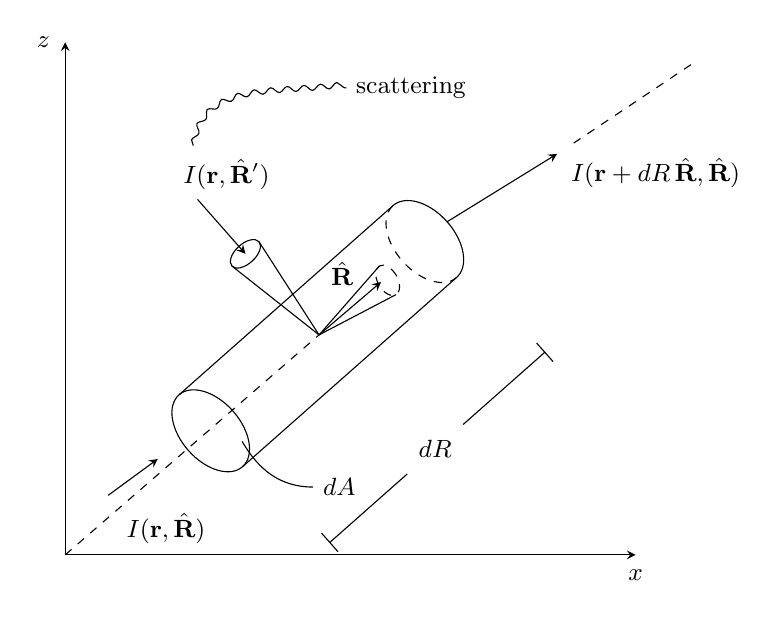
\begin{tikzpicture}[scale=1.05, >=stealth, font=\small]
		\def\ang{41.5}
		\coordinate (O) at (0,0);
		\coordinate (B) at (1.76,1.5);   % center of the bottom face
		\coordinate (Tp) at (4.35,3.79); % center of the top face
		\coordinate (Q) at (3.07,2.66);  % scattering point on the axis
		% axes
		\draw[->] (O) -- (0,6.2) node[anchor=east, xshift=-2pt] {$z$};
		\draw[->] (O) -- (6.9,0) node[anchor=north, yshift=-2pt] {$x$};
		% dashed line from the origin along the cylinder axis
		\draw[dashed] (O) -- (Q);
		% cylinder sides (tangent to the faces)
		\draw ($(B)+(\ang+90:0.58)$) -- ($(Tp)+(\ang+90:0.58)$);
		\draw ($(B)+(\ang-90:0.58)$) -- ($(Tp)+(\ang-90:0.58)$);
		% bottom face (solid) and top face (hidden half dashed)
		\draw[rotate around={\ang:(B)}] (B) ellipse (0.36 and 0.58);
		\draw plot[domain=-90:90, samples=60, smooth] ({4.35+0.36*cos(\x)*cos(\ang)-0.58*sin(\x)*sin(\ang)},{3.79+0.36*cos(\x)*sin(\ang)+0.58*sin(\x)*cos(\ang)});
		\draw[dashed] plot[domain=90:270, samples=60, smooth] ({4.35+0.36*cos(\x)*cos(\ang)-0.58*sin(\x)*sin(\ang)},{3.79+0.36*cos(\x)*sin(\ang)+0.58*sin(\x)*cos(\ang)});
		% incident brightness
		\draw[->] (0.52,0.72) -- (1.12,1.16);
		\node[anchor=north] at (1.22,0.62) {$I(\mathbf{r},\hat{\mathbf{R}})$};
		% dA
		\draw ($(B)+(\ang-60:0.4)$) to[out=-60, in=180] (3.0,0.82) node[anchor=west] {$dA$};
		% dR dimension line with end bars, broken at the label
		\coordinate (D1) at (3.2,0.15);
		\coordinate (D2) at (5.8,2.45);
		\draw (D1) -- ($(D1)!0.36!(D2)$);
		\draw ($(D1)!0.62!(D2)$) -- (D2);
		\draw ($(D1)+(\ang+90:0.15)$) -- ($(D1)+(\ang-90:0.15)$);
		\draw ($(D2)+(\ang+90:0.15)$) -- ($(D2)+(\ang-90:0.15)$);
		\node at ($(D1)!0.49!(D2)$) {$dR$};
		% emergent brightness
		\draw[->] ($(Tp)+(\ang:0.36)$) -- (5.95,4.85);
		\draw[dashed] (6.15,4.98) -- (7.6,5.95);
		\node[anchor=west] at (6.0,4.62) {$I(\mathbf{r} + dR\,\hat{\mathbf{R}}, \hat{\mathbf{R}})$};
		% cone of radiation scattered into the cylinder from direction R-hat'
		\coordinate (C1) at (2.18,3.64);
		\draw[rotate around={42.2:(C1)}] (C1) ellipse (0.22 and 0.12);
		\draw ($(C1)+(42.2:0.22)$) -- (Q);
		\draw ($(C1)+(222.2:0.22)$) -- (Q);
		\draw[->] (1.6,4.3) -- (C1);
		\node[anchor=south] at (1.95,4.3) {$I(\mathbf{r},\hat{\mathbf{R}}')$};
		\node[anchor=west] at (3.4,5.65) {scattering};
		\draw[decorate, decoration={snake, amplitude=1pt, segment length=6pt}] (1.55,4.95) to[out=80, in=190] (3.4,5.65);
		% cone scattered into direction R-hat
		\coordinate (C2) at (3.9,3.32);
		\draw[rotate around={30:(C2)}, dashed] (C2) ellipse (0.12 and 0.2);
		\draw (Q) -- ($(C2)+(120:0.2)$);
		\draw (Q) -- ($(C2)+(-60:0.2)$);
		\draw[->] (Q) -- (3.82,3.3);
		\node at (3.35,3.4) {$\hat{\mathbf{R}}$};
	\end{tikzpicture}
	\caption{Radiative transfer through an infinitesimal cylinder of cross-sectional area $dA$ and length $dR$ at position $\mathbf{r}$, for propagation in direction $\hat{\mathbf{R}}$; radiation incident from direction $\hat{\mathbf{R}}'$ is scattered into $\hat{\mathbf{R}}$ (cf.\ Ulaby and Long (2014), Fig.~6-12).}
	\label{f:cyl}
\end{figure}
% NOTE: the caption is added.

% NOTE (page L9): handwritten units [W/m^2] (twice) corrected to [W m^-2 sr^-1]: the brightness (brightness intensity,
% or radiance) is a power per unit area per unit solid angle (U&L 2014, Table 6-1, p. 228: "watt per steradian per
% square meter"; p. 241: "energy per unit area dA, radiated within a solid angle dOmega, during an interval of 1 s";
% Liou 2002, Eq. 1.1.7, p. 4); in the Rayleigh-Jeans form of Eq. (e:I), P_bb/lambda^2 = P_bb/(A_eff Omega_p) is
% per steradian. (As in U&L, I is integrated over the bandwidth Delta f; Liou's I_lambda is monochromatic.)
% NOTE: handwritten I(r + dR, R-hat); corrected to I(r + dR R-hat, R-hat), because r is a vector and dR a length
% (U&L 2014, p. 241, write I(R + dR, R-hat) with bold R and dR).
% NOTE: the word "brightness" in the first definition is written over or struck through in the scan (low-confidence
% reading); transcribed as "brightness", as in the other two definitions and on page L10.
\begin{itemize}
	\item[] $I(\rv,\Rh) \equiv$ incident brightness at position $\rv$ in direction $\Rh$ $\left[\dfrac{\text{W}}{\text{m}^2\,\text{sr}}\right]$
	\item[] $I(\rv + dR\,\Rh, \Rh) \equiv$ brightness of EM radiation leaving cylinder $\left[\dfrac{\text{W}}{\text{m}^2\,\text{sr}}\right]$
	\item[] $I(\rv,\Rh') \equiv$ brightness of EM radiation scattered into the cylinder from surrounding area
\end{itemize}

% ---- page L10 ----
\begin{itemize}
	\item Power (brightness) leaving cylinder is $<$ that entering cylinder due to extinction (scattering + absorption)
	% NOTE: checked against U&L 2014, Eqs. 6.45-6.46 (p. 241) and Lecture 9 (Eq. e:ke there; kappa_a = -2 k_0 Im{sqrt
	% eps} = 2 alpha). No polarization index on the kappas here (as kappa_a in Lecture 11). Handwritten K_0 written k_0
	% (D14). The two handwritten arrows from kappa_s and kappa_a to their descriptions are set as the two lines below
	% the equation.
	\item The change from incident brightness $I(\rv,\Rh)$ due to extinction is
	\begin{equation}
		\label{e:dIext}
		dI_\mathrm{extinction} = \ke I(\rv,\Rh)\,dR
	\end{equation}
	where
	\begin{align*}
		\ke &\equiv \text{extinction coef (introduced in Lecture~9)}\\
		&= \ka + \ks
	\end{align*}
	\begin{itemize}
		\item[] $\ks$: \ $\hookrightarrow$ scattering coef
		\item[] $\ka$: \ $\hookrightarrow$ absorption coef $= -2k_0\,\mathrm{Im}\{\sqrt{\varepsilon}\}$
	\end{itemize}
	% NOTE: checked against U&L 2014, Eqs. 6.47, 6.51 (p. 242). The handwritten "J = is total source function" is read
	% as "J = total source function" ("is" squeezed after the identity sign; low-confidence reading). J is flagged
	% against the rotational quantum number J (L10, L11) in master table D149.
	\item Media inside cylinder emits EM radiation w/ brightness
	\begin{equation}
		\label{e:dIem}
		dI_\mathrm{emission} = \ke J(\rv,\Rh)\,dR
	\end{equation}
	where
	\begin{itemize}
		\item[] $J \equiv$ total source function
	\end{itemize}
\end{itemize}

% ---- page L11 ----
\begin{itemize}
	% NOTE: checked against U&L 2014, Eqs. 6.47-6.52 (p. 242): J = (1 - a) J_a + a J_s, a = kappa_s/kappa_e. The
	% subscript e of kappa_e in the denominator is typed in the scan. a is flagged in master table D148.
	\item Total source function $J$ is a weighted sum of scattering $J_\mathrm{s}$ and absorption (emission) $J_\mathrm{a}$ source functions
	\begin{equation}
		\label{e:J}
		J = (1 - a)J_\mathrm{a} + aJ_\mathrm{s}
	\end{equation}
	where
	\begin{equation*}
		a = \frac{\ks}{\ke} \equiv \text{single-scatter albedo}
	\end{equation*}
	\begin{itemize}
		% NOTE: checked against U&L 2014, Eq. 6.48 (p. 242): J_s = (1/kappa_s) times the integral over 4 pi of
		% psi(R-hat, R-hat') I(R, R-hat') dOmega'.
		\item[] $J_\mathrm{s} \equiv$ scattering source function: accounts for radiation scattered along $\Rh$ (by matter in cylinder) and sourced from EM radiation coming in from all directions (e.g., sunlight scattered by surrounding atmosphere)
		% NOTE: checked against U&L 2014, p. 242 (Kirchhoff's law under local thermodynamic equilibrium; radiometer
		% integration times of milliseconds to seconds) and Liou 2002, Sec. 1.2.4 (p. 13). "Kirchoff's" (handwritten)
		% corrected to "Kirchhoff's" (Gustav Kirchhoff), here and on page L13.
		\item[] $J_\mathrm{a} \equiv$ absorption source function: emission must balance absorption when matter is in thermal equilibrium (Kirchhoff's Law of thermal radiation) $\rightarrow$ In RS, this is a reasonable approx.\ under local thermodynamic equilibrium (collision-dominated; in Earth's atmosphere below ${\sim}60$--$70$~km; Liou, 2002, pp.~14, 27)
		% NOTE: handwritten reads "In RS, timescales are sufficiently short that this is a reasonable approx."; changed
		% to "under local thermodynamic equilibrium (...)" because Kirchhoff's law holds where molecular collisions
		% dominate over radiative transitions, not because of the radiometer's integration time: Liou 2002, p. 14 ("in
		% a localized volume below about 60-70 km ... energy transitions are governed by molecular collisions. It is
		% in the context of this local thermodynamic equilibrium (LTE) that Kirchhoff's law is applicable") and p. 27
		% (the non-LTE level "occurs at about 60-70 km") (instructor decision 2026-09-30).
	\end{itemize}
\end{itemize}

%%%%%%%%%%%%%%%%%%%%%%%%%%%%%%%%%%%%%
% ---- page L12 ----
% NOTE: subsection heading added.
\subsection{Radiative transfer equation}
\label{s:rte}

\begin{itemize}
	% NOTE: checked against U&L 2014, Eq. 6.53 (p. 242). The labels "source" and "sink" with their arrows are
	% handwritten.
	\item Now, propagation over distance $dR$ results in change of (power) intensity $dI$
	\begin{align}
		dI &= \overset{\substack{\text{source}\\\swarrow}}{dI_\mathrm{emission}} - \overset{\substack{\text{sink}\\\swarrow}}{dI_\mathrm{extinction}} \nonumber\\
		&= \ke J\,dR - \ke I\,dR \nonumber\\
		&= \ke\,dR\left[J(\rv,\Rh) - I(\rv,\Rh)\right] \label{e:dI}
	\end{align}
	% NOTE (page L12): handwritten tau (optical depth) written tau_opt, because tau is the Fresnel transmission
	% coefficient (instructor decision D18) (following the gamma_st precedent, D66; formerly F2, now master table
	% D137). Checked against U&L 2014, Eqs. 6.54-6.55 (p. 242): d tau = kappa_e dR, with tau increasing along the
	% direction of propagation, and dI/d tau + I = J (the "radiative transfer equation"). Liou 2002 (Eq. 1.4.5,
	% p. 28) writes the same equation as dI/(k rho ds) = -I + J; his optical thickness (Eq. 1.4.16, p. 30) is
	% measured backward from the far end s_1, d tau = -k rho ds, which flips the sign of the derivative (Eq. 1.4.17).
	% Handwritten "radiative transfer function" written "radiative transfer equation", as in U&L and Liou (instructor
	% decision, 2026-09-30); also at the "Plugging into" line below. The box is handwritten.
	\item Defining optical depth $d\topt = \ke\,dR$, we can rearrange to get the radiative transfer equation
	\begin{equation}
		\label{e:RTE}
		\boxed{\frac{dI}{d\topt} + I = J}
	\end{equation}
	% NOTE: "incident brightness temperature" kept as handwritten; the equation is written for the brightness I, which
	% is proportional to the brightness temperature (Eq. e:I; U&L 2014, p. 235: T_B is used as a surrogate for I);
	% the form in T_B is Eq. (e:RTETB).
	\item[] In words: Change in brightness w/ optical depth (product of $\ke$ and $dR$) $=$ total source less incident brightness temperature
	\begin{itemize}
		\item[$\hookrightarrow$] In essence, statement of conservation of energy
	\end{itemize}
\end{itemize}

%%%%%%%%%%%%%%%%%%%%%%%%%%%%%%%%%%%%%
% ---- page L13 ----
% NOTE: subsection heading added.
\subsection{Radiative transfer in terms of brightness temperature}
\label{s:rtetb}

\begin{itemize}
	\item Relating to brightness temperature $T_\mathrm{B}$
	\begin{itemize}
		% NOTE: checked against U&L 2014, Eqs. 6.56-6.58 (p. 243) (one polarization; see the NOTE at Eq. e:I).
		\item[] Recall Rayleigh--Jeans
		\begin{equation}
			\label{e:ITB}
			I = \frac{k_B}{\lambda^2}\,\Delta f\,T_\mathrm{B}
		\end{equation}
		\item[] By Kirchhoff's law, emission $=$ absorption
		\begin{equation}
			\label{e:Ja}
			\Rightarrow\quad J_\mathrm{a} = \frac{k_B}{\lambda^2}\,\Delta f\,T \qquad T = T(\rv)
		\end{equation}
		\begin{itemize}
			\item[$\hookrightarrow$] $J_\mathrm{a}$ is isotropic $\Rightarrow$ $J_\mathrm{a} = J_\mathrm{a}(\rv)$
		\end{itemize}
		% NOTE: T_VS is flagged in master table D146.
		\item[] Analogously, define volume scattered radiometric temperature $T_\mathrm{VS}(\rv,\Rh)$ such that
		\begin{equation}
			\label{e:Js}
			J_\mathrm{s}(\rv,\Rh) = \frac{k_B}{\lambda^2}\,\Delta f\,T_\mathrm{VS}(\rv,\Rh)
		\end{equation}
		% NOTE: checked against U&L 2014, Eq. 6.60 (p. 243), dT_B/d tau + T_B = (1 - a) T + a T_VS, and by substituting
		% Eqs. (e:J), (e:ITB)-(e:Js) into Eq. (e:RTE) (the common factor k_B Delta f/lambda^2 cancels). Handwritten tau
		% written tau_opt (D137). The box is handwritten.
		\item[] Plugging into radiative transfer equation
		\begin{equation}
			\label{e:RTETB}
			\boxed{\frac{dT_\mathrm{B}}{d\topt} = (1 - a)T + aT_\mathrm{VS} - T_\mathrm{B}}
		\end{equation}
	\end{itemize}
\end{itemize}

%%%%%%%%%%%%%%%%%%%%%%%%%%%%%%%%%%%%%
% Symbols follow the master table in ../variables_master.tex; see it for flagged dual usages.
\clearpage
\section*{Variables}

Units are SI. Values are given for universal constants. The brightness $I$ (from Section~\ref{s:tb} on) is the brightness of one polarization integrated over the bandwidth $\Delta f$ (Rayleigh--Jeans form, Eq.~\eqref{e:I}).

{\small
\renewcommand{\arraystretch}{1.2}
\begin{longtable}{>{$}l<{$} >{\raggedright\arraybackslash}p{0.38\textwidth} >{\raggedright\arraybackslash}p{0.16\textwidth} >{\raggedright\arraybackslash}p{0.19\textwidth}}
\hline
\textrm{Symbol} & Description & Units & Value \\
\hline
\endfirsthead
\hline
\textrm{Symbol} & Description & Units & Value \\
\hline
\endhead
\hline
\endfoot
\multicolumn{4}{l}{\emph{Constants}} \\*
c & speed of light in a vacuum & m/s & $2.998\times10^{8}$ \\
h & Planck constant & J\,s & $6.63\times10^{-34}$ \\
k_B & Boltzmann constant & J/K & $1.38\times10^{-23}$ \\
\sigma_\mathrm{SB} & Stefan--Boltzmann constant & W\,m$^{-2}$K$^{-4}$ & $5.67\times10^{-8}$ \\
\multicolumn{4}{l}{\emph{Black body radiation and received power}} \\*
T & (absolute, physical) temperature & K & -- \\
f & frequency, $\omega/2\pi$ & Hz & -- \\
\omega & angular frequency & rad/s & -- \\
\lambda & wavelength & m & $c/f$ \\
B_f & spectral radiance (per unit frequency) & W\,m$^{-2}$ sr$^{-1}$ Hz$^{-1}$ & -- \\
B_\lambda & spectral radiance (per unit wavelength) & W\,m$^{-2}$ sr$^{-1}$ m$^{-1}$ & -- \\
\lambda_\mathrm{max} & wavelength of the peak of $B_\lambda$ (Wien) & m & ${\propto}T^{-1}$ \\
z & $hf/(k_BT)$ & dimensionless & RJ: $z \ll 1$ \\
A_\mathrm{s} & area of the black-body source & m$^2$ & -- \\
\Aeff & (effective) area of the receiving antenna & m$^2$ & $\lambda^2/\Omega_\mathrm{p}$ \\
R & distance between source and antenna & m & -- \\
\Omega, d\Omega & solid angle; its differential & sr & -- \\
\Omega_\mathrm{r} & solid angle subtended by the antenna at the source & sr & $\Aeff/R^2$ \\
\Omega_\mathrm{s} & solid angle subtended by the source at the antenna & sr & $A_\mathrm{s}/R^2$ \\
P_f & spectral power received & W/Hz & -- \\
P & total power received & W & -- \\
f_\mathrm{low}, f_\mathrm{high} & lower and upper limits of the receiver band (also $f_1$, $f_2$) & Hz & -- \\
\Delta f & bandwidth & Hz & $f_\mathrm{high} - f_\mathrm{low}$ \\
% NOTE: added (instructor decision 2026-09-30): row for L (used in the text at Eq. e:SB), and "= pi L" in the I row.
L & total radiance of a black body (Lecture~12) & W\,m$^{-2}$sr$^{-1}$ & $\sigma_\mathrm{SB}T^4/\pi$ \\
I & (Eq.~\ref{e:SB}) intensity (flux density) of a black body, $\pi L$ & W/m$^2$ & $\sigma_\mathrm{SB}T^4$ \\
\multicolumn{4}{l}{\emph{Antenna}} \\*
F(\theta,\phi) & (normalized) radiation pattern of the antenna & dimensionless & max.\ 1 \\
\theta, \phi & colatitude and longitude (spherical coordinates) & rad & -- \\
x, y, z & Cartesian coordinates (figures) & m & -- \\
c_p & polarization factor of the antenna & dimensionless & 1 (non-polarized), $\frac12$ (polarized) \\
\Omega_\mathrm{p} & antenna pattern solid angle, $\iint_{4\pi}F\,d\Omega$ & sr & $\lambda^2/\Aeff$ \\
P_\mathrm{bb} & power received from a black body & W & $k_BT\Delta f$ ($c_p = \frac12$) \\
\multicolumn{4}{l}{\emph{Brightness and emissivity}} \\*
I(\theta,\phi) & brightness (intensity) of a material (one polarization) & W\,m$^{-2}$sr$^{-1}$ & $k_B\Delta f\,T_\mathrm{B}/\lambda^2$ \\
I_\mathrm{bb} & brightness of a black body & W\,m$^{-2}$sr$^{-1}$ & $k_B\Delta f\,T/\lambda^2$ \\
P(\theta,\phi) & power received from a material & W & -- \\
e(\theta,\phi) & emissivity & dimensionless & $0$--$1$ \\
T_\mathrm{B} & brightness temperature & K & $eT$ \\
\multicolumn{4}{l}{\emph{Radiative transfer}} \\*
\mathbf{r} & position vector & m & -- \\
\hat{\mathbf{R}}, \hat{\mathbf{R}}' & direction of propagation; direction of radiation scattered into $\hat{\mathbf{R}}$ & dimensionless & -- \\
dA, dR & cross-sectional area and length of the cylinder & m$^2$; m & -- \\
I(\mathbf{r},\hat{\mathbf{R}}) & brightness at $\mathbf{r}$ in direction $\hat{\mathbf{R}}$ & W\,m$^{-2}$sr$^{-1}$ & -- \\
dI_\mathrm{extinction} & loss of brightness by extinction over $dR$ & W\,m$^{-2}$sr$^{-1}$ & $\ke I\,dR$ \\
dI_\mathrm{emission} & gain of brightness by emission over $dR$ & W\,m$^{-2}$sr$^{-1}$ & $\ke J\,dR$ \\
\ke & extinction coefficient & Np/m & $\ka + \ks$ \\
\ka & absorption coefficient & Np/m & $-2k_0\,\mathrm{Im}\{\sqrt{\varepsilon}\}$ \\
\ks & scattering coefficient & Np/m & -- \\
k_0 & free-space wavenumber & rad/m & $2\pi/\lambda$ \\
\varepsilon & complex dielectric constant & dimensionless & -- \\
J & total source function & W\,m$^{-2}$sr$^{-1}$ & $(1-a)J_\mathrm{a} + aJ_\mathrm{s}$ \\
J_\mathrm{a} & absorption source function & W\,m$^{-2}$sr$^{-1}$ & $k_B\Delta f\,T/\lambda^2$ \\
J_\mathrm{s} & scattering source function & W\,m$^{-2}$sr$^{-1}$ & $k_B\Delta f\,T_\mathrm{VS}/\lambda^2$ \\
a & single-scattering albedo & dimensionless & $\ks/\ke$ \\
\topt & optical depth, $\int\ke\,dR$ & Np (dimensionless) & -- \\
T_\mathrm{VS} & volume scattered radiometric temperature & K & -- \\
\end{longtable}
}

\end{document}
